\documentclass[12pt]{ctexart}%中文包
\usepackage{graphicx}%图片引用包
\usepackage{amssymb}%特殊符号
\usepackage{amsmath,amsfonts,bm}%矩阵
\usepackage{amsthm}%定理
\usepackage{geometry}%缩放
\usepackage{hyperref}%超链接
\usepackage{framed}%框框
\usepackage{color}%颜色
\usepackage{mathrsfs}%花体
\usepackage{anyfontsize}
\usepackage{indentfirst}%缩进
\usepackage{extsizes}%size
\usepackage{newtxtext,newtxmath}%times风格字体
\usepackage{mdframed}%边栏
\usepackage{enumerate}
\usepackage{braket}

\surroundwithmdframed[
  linecolor=gray,
  topline=false,
  bottomline=false,
  rightline=false,
  linewidth=4pt,
  innerleftmargin=10pt,
  innerrightmargin=10pt,
  innertopmargin=0pt,
  innerbottommargin=5pt
]{theorem}
\surroundwithmdframed[
    linecolor=black,
    leftline=false,
    rightline=false,
    linewidth=0.5pt,
    innerleftmargin=10pt,
    innerrightmargin=10pt,
    innertopmargin=0pt,
    innerbottommargin=5pt
]{note}

\newtheorem{theorem}{Theorem}
\newtheorem{note}{Note}
\geometry{a4paper,scale=0.85}
\hypersetup
    {
        hypertex=true,
        colorlinks=true,
        linkcolor=blue,
        anchorcolor=blue,
        citecolor=blue
    }


\title{Basis of Single Molecular Localization Microscopy\\单分子定位超分辨成像技术基础}

\author{Jerry Ling} 

\date{\today}
 
\begin{document}  %begin后括号内是文件类型
\maketitle  %生成标题
SMLM是一种利用特殊的染料设计在普通宽场显微镜下实现超分辨成像的技术。其染料分子通常具有自行闪烁、受激切换(stochastic optical reconstruction microscopy, STROM; fluorescence photoactivated localization microscopy, PALM)或解离-连接平衡(Point accumulation in nanoscale topography, PAINT)的特性。得益于此,标记点(label)将在不同时间亮起而避免了衍射斑重叠。识别单分子信号后,通过近似的高斯拟合可以定位其坐标,通过多帧合并获得超分辨(20-50nm)图像。本笔记基于综述文献,将逐一细察荧光染料及亮暗态切换原理、标记策略、设备搭建和数据、分辨率分析。\begin{figure}[t] %two figures
    \centering
    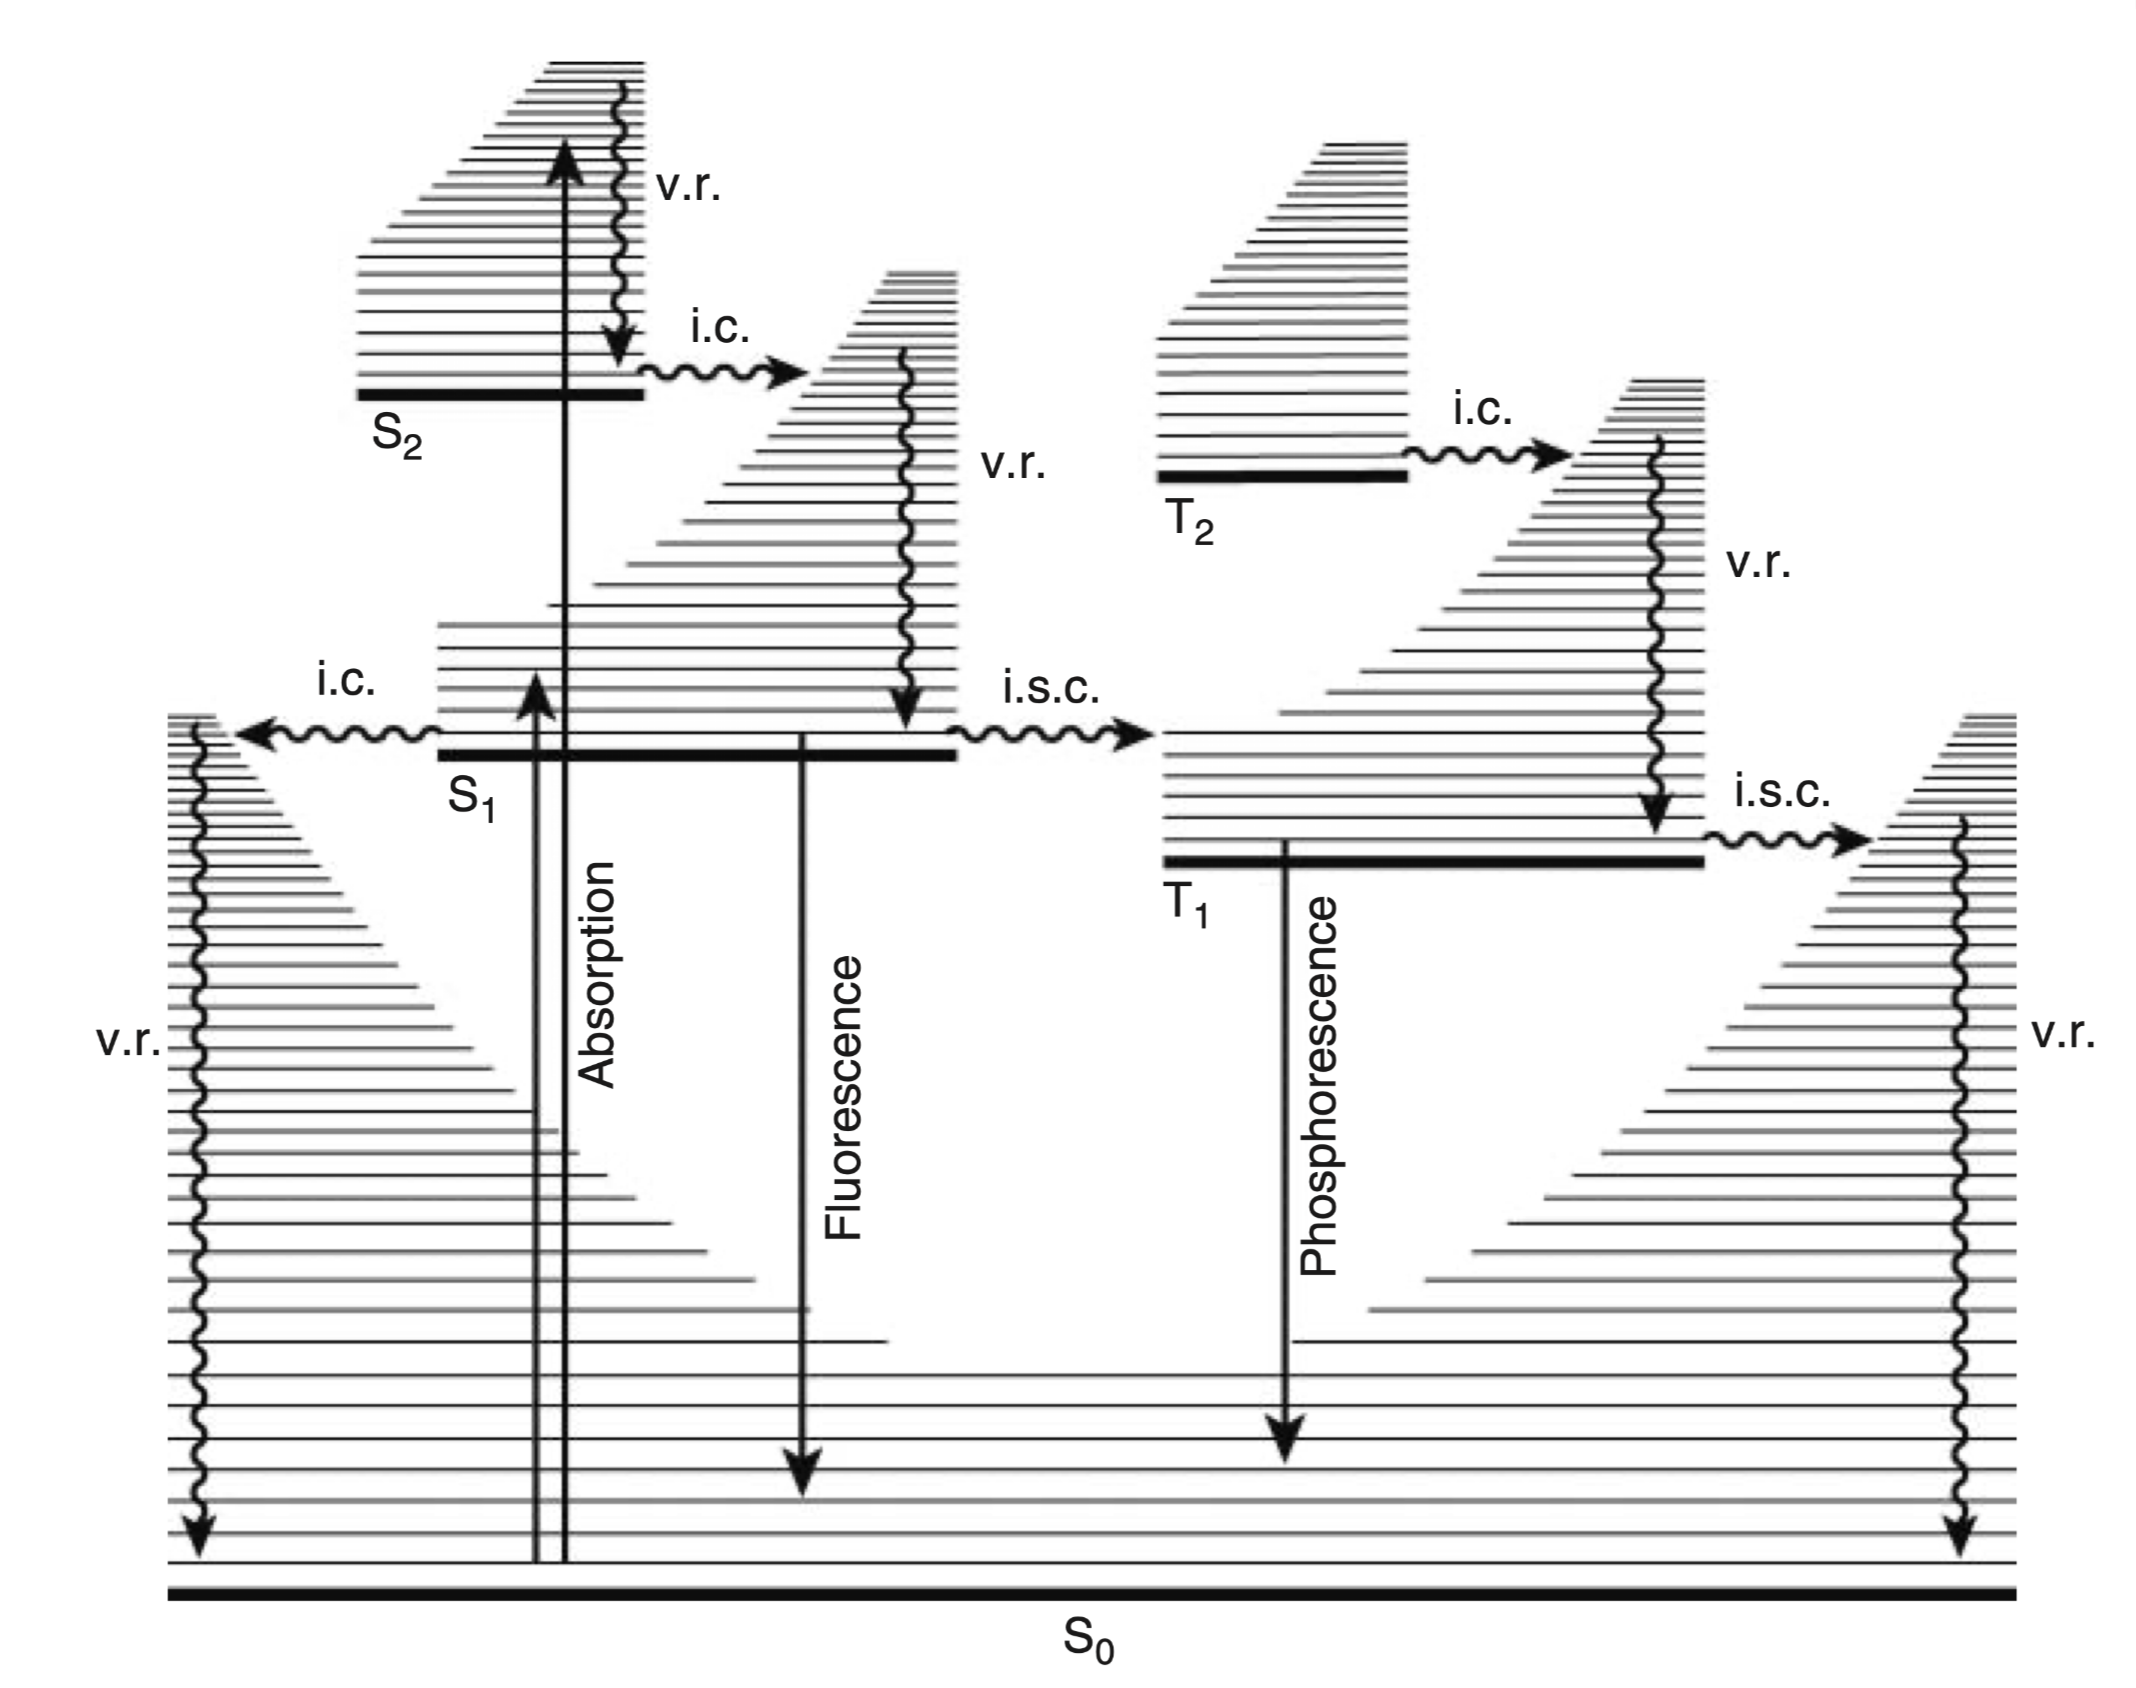
\includegraphics[width=0.6\textwidth]{Kinetic_diagram}
    \caption{Kinetic Diagram of Fluorescence Molecular}
    \label{Kinetic}
\end{figure}
\section*{开关:光反应的控制艺术}
根据超分辨成像的需求,考虑能够在\textbf{亮态(ON)}和\textbf{暗态(OFF)}间转化的荧光分子:
\begin{framed}
    \begin{enumerate}[a)]
        \item 在两态间可逆转换(存在平衡),即自发闪烁
        \item 原本不发光,通过激光(UV)部分激活,在最大吸收光作用下发生光漂白(PALM)
        \item 原本可发荧光,在最大吸收光作用下生成长时间稳定的暗态,且能通过激光(UV/活化分子传递)激活至亮态(STROM)
    \end{enumerate}
\end{framed}
\noindent 其中态间的转化的光物理/光化学过程决定了其特性和调控的方式。下面简要回顾荧光的基本过程:
\subsection*{荧光基本过程和概念}
\par 分子的荧光过程可参考图\ref{Kinetic}示意。基态($S_0$)的电子在激发光作用下发生跃迁,进入激发态($S_1$)的某振动能级上(Frank-Condon原理)。其跃迁速率可通过微扰理论导出:
\begin{equation}
    \omega(if)=\omega(fi)\propto \rho(\mu_{if})\bra{i}\hat{\mu}\ket{f}^2
    \label{pert}
\end{equation}
其中i和f表示始、终态,$\rho$指对应能级差的\textbf{辐射密度},$\bra{i}\hat{\mu}\ket{f}$是跃迁\textbf{矩阵元(transition moment)},两态间的算符是偶极矩算子。注意到两个方向的跃迁几率一致,分别称为\textbf{受激吸收(induced absorption)}和\textbf{受激发射(induced emission)}。后者与激发光同相同向,对我们而言不重要。该过程使能级布局数偏离统计平衡态,被激发的电子需要以某种方式返回平衡态:
\begin{itemize}
    \item 振动弛豫(vibrational relaxation, v.r.):非辐射过程,很快,使得激发到S1振动能级上的电子快速返回S1振动基态
    \item 内转换(internal conversion, i.c.):非辐射过程,自旋不变转换至电子基态的高振动能级上,而后立刻进入振动弛豫
    \item \textbf{自发辐射(spontaneous emission)}:各向同性的发光,由图可见其波长一般大于吸收光,即通常意义上的\textbf{荧光(fluorescence)}。
    \item \textbf{系间穿越(intersystem crossing, i.s.c.)}:由单线态向附近三线态转移的非辐射过程。通常自旋禁阻,但在有机染料分子中常见(n,$\pi^*有轨道存在$)。这步过程是不少有机染料闪烁的重要步骤。若三线态辐射跃迁回基态,所发出的光一般称为磷光,寿命通常大大高于荧光($10^{-4}s$ v.s $10^{-7}s)$。
\end{itemize}
在我们的问题中,染料(如Cy5)具有较大的系间穿越速率。而在体系中加入巯基等还原剂($\beta$-ME)能进一步形成稳定的加合物,即出现长时间的\textbf{暗态}(寿命可达数小时)。然而其中涉及复杂的光物理和光化学过程(如单光子参与的光电子传递反应,photoelectron transfer),其机理尚待更多研究阐明。
\par 除了上述光物理过程和还原剂参与反应外,处理荧光分子还另需考虑\textbf{光漂白(photobleaching,不可逆光反应)}的问题。如体系中的氧气是常见的导致光漂白的物质,在需要的情况下必须进行除氧处理。
\begin{note}[lifetime explaned]
    处理荧光染料特性时候各种寿命容易混淆,特此说明较重要的几种参数:
    \begin{itemize}
        \item 荧光寿命:指$S_1$态的寿命,因为对环境的敏感性常用于荧光寿命成像(见本目录另一篇note)。实验上通过脉冲激发后测量时间分辨的光子数获得指数衰减的曲线拟合得到:\[\tau=\frac{1}{k_{F}+k_{ST}+k_{relax}}\]
        \item 亮态寿命:指在持续激发下亮态的寿命,可能是光漂白或暗态转化所致。与荧光寿命不同的是,亮态寿命通常和\textbf{激发光强度}有关,因为其反应通常涉及光子。
        \item 暗态寿命:概念同亮态相似。测量亮暗态寿命可以直接记录荧光强度进行指数拟合,也可进行单分子“轨迹”分析,见下节。
    \end{itemize}
    P.S.(荧光寿命光强无依赖性)由式(\ref{pert})可看出,激光强度影响仅激发几率,也即影响能级布局。布局数增加则会间接影响荧光\textbf{发射强度},但不影响荧光寿命,因为光子不参与自发辐射过程(若光强足够大则属于非线性光学,需另作考虑):
    \[I_{f}=N_{S_1}k_{F}\]
\end{note}


\subsection*{常用的开关分子及其典型信号}
\begin{figure}[b] %two figures
    \centering
    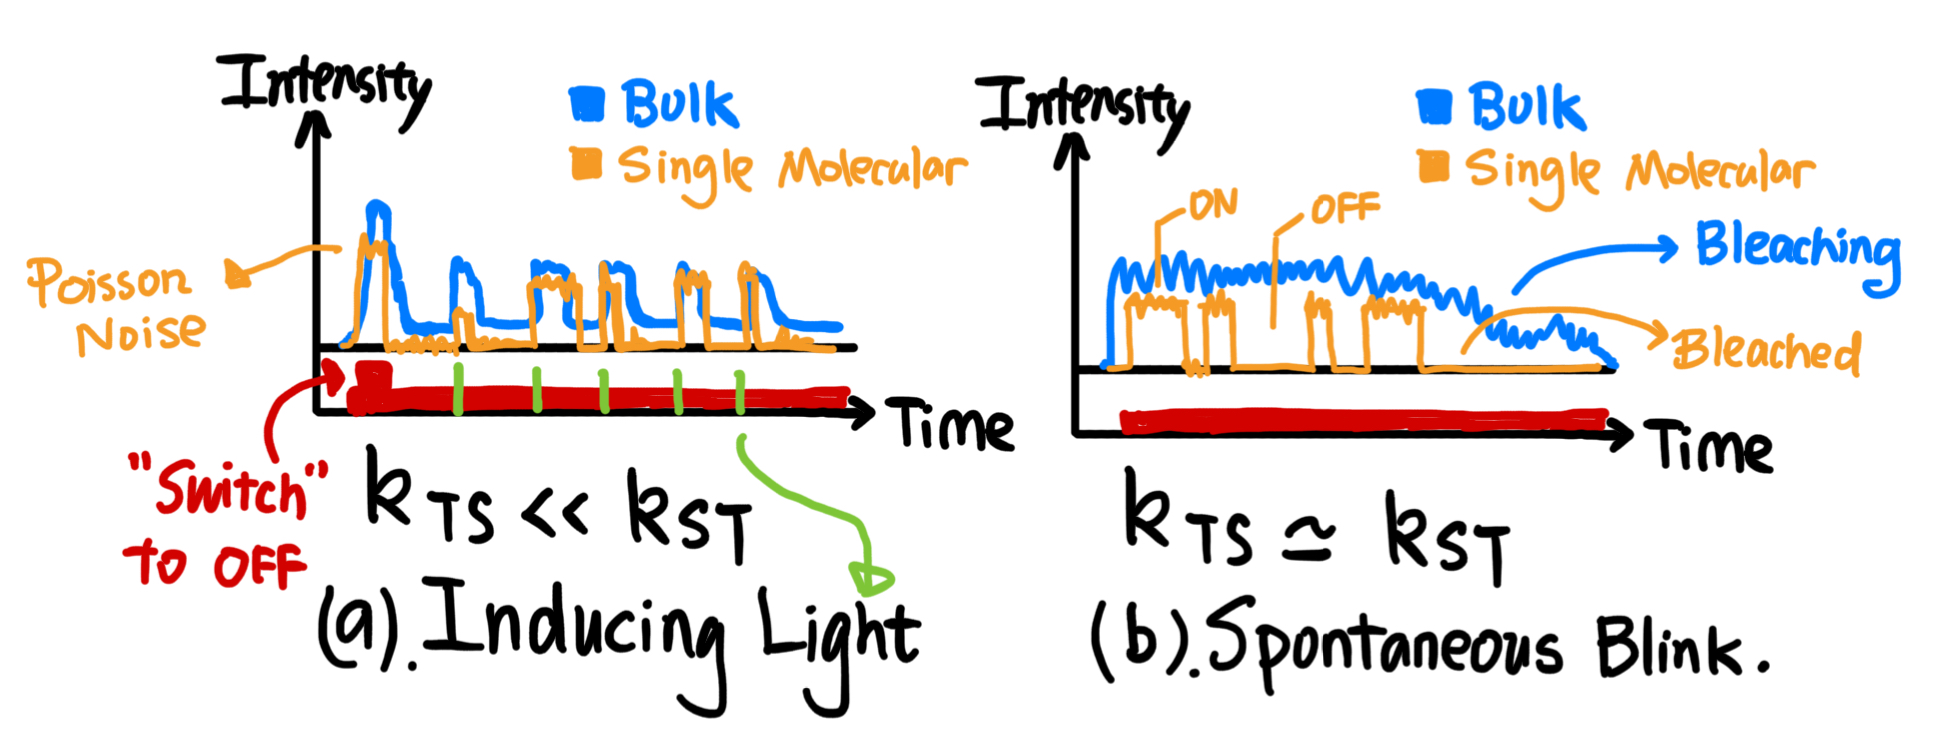
\includegraphics[width=0.8\textwidth]{Dynamic_diagram.jpeg}
    \caption{Intensity of Bulk and Single Molecule w.r.t. Time}
    \label{Dynamic}
\end{figure}
在显微镜下,我们有研究单分子发射信号的能力。考察每一个单分子的状态,则不难发现其反应的过程是一个基于一定参数的随机过程。若体系宏观上是均匀的,那么对单分子行为进行统计就能获得一个无偏的宏观动力学估计器。下面对常用的荧光分子进行介绍,并给出其典型的单分子和整体信号(见图\ref{Dynamic})。
\begin{enumerate}[i)]
    \item 光开关:Cy5,Alexa Fluor 647;Alexa Fluor dyes,ATTO dye。典型条件PBS+10-100nM$\beta$-ME+enzymatic oxygen scavenger。控制氧气-还原剂\textbf{含量}和\textbf{激发光强度}可以控制亮态(5-20ns)暗态(seconds)寿命。暗态到亮态到激活可用紫外(405nm)或邻近的激发分子(Cy3)。每次控制激发的数量以保证不重叠并减少光漂白是成功成像的关键。
    \item 光激活:photochromic rhodamine amides30, Janelia Fluor® 549, PA Janelia Fluor® 646,Cy5B。UV激活,但在下一次激活前需要用较长波长光漂白。荧光蛋白有PAmCherry,PA-TagRFP,PA-GFP等。亮态被淬灭前的光子数决定了单帧定位精度,但较长的寿命也降低了帧率。
    \item 光转换:Eos,Dendra2,mMaple。紫外光可令其荧光颜色转化(Eos:488-561nm),如同光激活染料,需要漂白掉转化的分子后再进行下一次转化。
    \item 自发闪烁:HMSiR39,HEtetTFER40,RD。其闪烁源于化学反应而同激发强度无关,常通过pH调节其速率,可用于live cell成像。
\end{enumerate}
注意图\ref{Dynamic}每个周期中单分子进入暗态的时间是一个随机分布,而bulk中荧光衰减则是相同的。实验中暗态时可用较弱的激发光来“关闭”进入亮态的分子。“T”代表暗态,可能是三线态加合物,也可能是其他不发光的产物。
\section*{分辨率:标记、激发、光子数}
由于流程较长,超分辨成像的分辨率估计也较为复杂。首先,如果所有发射荧光的单分子都能精准定位,那么其分辨能力取决于\textbf{标记密度(labeling density)}。根据采样定理等分析,分辨频率最多达到标记密度的[5倍奈奎斯特频率],定义为采样频率的五分之一(分辨率R单位m,频率$\nu$单位$m^{-1}$,间距$\Delta$单位m):
\begin{equation}
    R\geq R_{5*Nyq}\triangleq[\frac{\nu_{sample}}{5}]^{-1}=5\Delta_{sample}
\end{equation}
譬如欲达到23nm的分辨率,则平均每4.6nm就应有一个标记分子被定位以达到该要求(P.S.标准\textbf{奈奎斯特频率}定义为采样频率的一半)。注意,合成图片的帧最好能将所有荧光分子locate至少一遍,或者located分子密度应当大于$R_{5*Nyq}$。
\par 其次,实际一定曝光时间的单分子不总是能准确、精确定位。若定位是无偏的,则一般认为分辨率还被其\textbf{精度(precision)}限制:
\begin{equation}\label{CRLB}
    R\geq R_{loc}\triangleq2.3\sigma_{loc}
\end{equation}
单分子发射的光子坐标(\textbf{点源扩散函数,PSF})本身应是一个近似的高斯分布的随机变量$N[(x,y),\sigma_0^2]$。我们实际上利用了N个样本(光子)在CMOS上的信号去估计该随机变量的坐标参数(x,y)。根据估计理论,估计器($\hat{x}$,$\hat{y}$)的方差必然大于其\textbf{MLE估计器}(最大似然估计)的方差:
\begin{theorem}[Cramér–Rao lower bound]
    \[Var(\hat{x})\geq-[\mathbb{E}\frac{\partial^2}{\partial x^2}\ln{p(L,x)}]^{-1}\]
\end{theorem}
其中p(L,x)指当\textbf{参数}为x时候观察到L的概率,也就是L取所有样本值时的联合概率密度分布。代入高斯分布,因为每个样本都是独立等同分布,可简化为:
\begin{equation}
    \sigma_{loc}\geq \frac{\sigma_0}{\sqrt{N}}
\end{equation}
注意,这个估计总是过于保守,且不考虑连接分子时导致的\textbf{偏差(bias)}。
\par 当取得了图像后,可以通过\textbf{傅立叶环相关分析(Fourier Ring Coreelation)}估计分辨率。通过比较两张图在频域某半径为r的环内的相关性,得到图像在某一截止空间频率内的“稳定性”,以同时考虑精度和采样。而实验中最常用的分辨率确定方法还是直接分辨\textbf{已知距离的生物结构}。
\par 最后,当应用于\textbf{时间分辨}的成像如活细胞成像时,每张超分辨图像的成像总时间应当远小于生物动态的进行时间。实验上将所有帧分组合成视频以实现动态成像。
\section*{实验:标记、固定和光路搭建}
将荧光开关的基团/分子引入观测的对象是SMLM的第一步。\textbf{目标蛋白(target protein)}指希望标记上荧光基团的蛋白。不同标记方法也会引入不同的\textbf{连接误差(link error)}。可通过以下方法实现:
\begin{itemize}
    \item 编码荧光蛋白 Encoding fluorescent proteins:通过转染融合了荧光蛋白基因的目标蛋白基因来表达能发射荧光的目标蛋白。好的选择应减少荧光蛋白对目标蛋白功能的影响。
    \item 免疫标记 Immunolabelling:合成染料无法直接编码,需要先耦合到能够结合目标蛋白的抗体上,或耦合到能够连接到一抗的二抗上。后者能有较强的荧光强度,但也引入更大的连接误差。通常不适用🆚活细胞成像(需要穿透细胞膜)。
    \item 蛋白标签 Protein tag:为目标蛋白编码进特殊的基序(motif)以特异性地连接合成染料上的配体。具有最小的连接误差。
    \item 直接标记 Direct labelling:使用连接了染料的肽段或药物直接标记肌动蛋白或微管。尽管很小,但会降低生物活性而作为修饰剂。若染料修饰了脂类分子则可直接整合进生物结构中。基因编码允许引入特殊氨基酸,如能和TCO反应的赖氨酸,TCO-lys复合物和同生物正交试剂发生\textbf{点击反应(click reaction)}从而引入荧光染料。
\end{itemize}
\par 对于需要固定的细胞或组织,希望保持其结合位点和蛋白作用。多聚甲醛PFA和戊二醛是最常用的交联剂,冰甲醇或乙二醇可用于细胞骨架固定和形态学研究。30分钟的4\% PFA和0.2\%glutar-aldehyde处理可抑制膜流动性以避免团簇。免疫标记法需要在固定后可渗透化,且需要在标记前加入BSA或NGS等blocking buffer以减少非特异性结合和背景噪音。此外,还可以用高压低温环境达到固定效果。而对于活细胞研究,细胞在PBS中被成像。\textbf{光毒性(Phototoxicity)}是需要考虑的因素,可用细胞分裂等方法测试之。
\par 成像只需要常用的传感器如EM-CCD和sCMOS,后者敏感性较低但允许帧率更高,其像素大小应接近衍射极限(150-200nm)。光路方面使用二色镜可以分离、合并两种颜色的激光,仔细调整可搭建多通道的系统。60–100x的油镜(N.A. 1.4)充当物镜以确保有效的光子收集。靠近盖玻片的样品可以使用\textbf{TIRF}来提升信噪比。使用特殊透镜调制信号可以实现\textbf{3d成像}。
\section*{数据处理和分析}
在SMLM中,每帧中亮起的分子应当在保证不重叠的条件下尽可能多,以尽快达到重构分辨率要求的帧数。开关分子的亮起由激光强度调控,且理论上可以使用反馈回路自动化,其曝光时间应接近ON-OFF的寿命(10-100ms)。用分辨率可以大致估计标记密度,用5-10倍的定位总数和每帧亮起的分子数估计总共需要的帧数,乘以曝光时间即总重构时间。
\par 时间分辨的结构动态成像方法见上文。跟踪单分子的方法则关注单分子的状态随时间的变化,称为\textbf{轨迹(trajectories)},以作为探针传递周围环境状态。此时标记密度不应过大以避免轨迹重叠,且应注意每帧曝光应选择使得单分子的位移大于定位精度。SMLM使得其能够同时定位几倍于单分子方法的分子轨迹,以展示细胞中的分子动态(如扩散速率分布)。
\par SMLM的数据处理按单分子检测、单分子定位和超分辨图像重构进行,其中重点如下:
\begin{itemize}
    \item 检测:检测前首先要\textbf{去除背景},可用算法rolling ball ,difference of Gaussians,滤波器, 背景平均扣除。接着单分子信号可以用同PSF的互相关搜寻(correlation)。噪声可来源于:暗电流,读出噪声(极少),光电子放大器噪声,泊松噪声。
    \item 定位精度:按式(\ref{CRLB})估计最小精度,典型光子数在$10^2-10^4$,$\sigma_0\approxeq100$nm。注意光学系统会导致PSF无法近似成高斯分布,背景噪声则会导致更差的精度。更好的精度估计公式参见:\textit{Kay, S. M. Fundamentals of Statistical Signal Processing Vol. 2: Detection Theory (Prentice Hall PTR, 1998).;Mortensen, K. I. el. Optimized localization analysis for single molecule tracking and super resolution microscopy. Nat. Methods 7, 377–381 (2010).}
    \item 定位算法:最大似然算法是所有算法的金标准,计算上通过迭代的梯度上升算法寻找最佳参数。PSF则常需要为每个实验单独标定以减少错误,更干净的背景能减少偏差。依靠图片处理单元,计算机现在已能够高效地完成这些任务。
    \item 后处理:可选择将邻近定位到的点合并为单个分子。另外,大部分SMLM实验需要进行\textbf{漂移矫正(drifting correction)},见后文。
    \item 重构:以上得到的坐标可以通过在亚像素(10nm)上显示来重构超分辨图像。每个点对应一定的像素亮度,经过线性叠加重构。
\end{itemize}
\par SMLM得到的数据可用于多种定量分析,如识别蛋白团簇、单分子计数、重建单个颗粒(需要该颗粒的多个相同成像)、多通道的共定位分析、单分子跟踪(Lagrangian/Eulerian)方法。其中许多技术来源于\textbf{空间统计学(spatial statistic)}。常用的软件包参见原始文献。
\end{document}
